\section{Vom linearen Modell zum Neuronalen Netz}

\subsection{Das Perceptron als additatives lineares Modell}
Eines der klassischsten Modelle der Regressionsanalyse sind lineare Regression und die logistic Regression. 

Es sind mathematisch simple Verfahren, die sogar analytisch lösbar sind - aber eben nicht immer ideale Ergebnisse erzielen: es gibt Probleme, die mit den Verfahren nicht lösbar sind. 

Eine Weiterentwicklung ist das so genannte Perceptron.
Eine gängige Definitition ist die, die auch in \cite{bishop1995neural} verwendet wird: 
Ein Perceptron besteht aus einem Eingabe-Vektor $x$, einem Gewichtsvektor $w$ und einem Bias-Wert $b$. Es ist ein binärer Klassifizierer, der das Ergebniss mit Hilfe der folgenden Formel berechnet:
\begin{equation}
\label{eq:perceptron}
    y = \begin{cases}
               1               & w x + b > 0.\\
               0               & \text{ansonsten}. %Das Satzzeichen hier ist etwas schwierig...
           \end{cases} 
\end{equation}

In dieser Formel entspricht $wx$ dem Skalarprodukt.

\subsection{Das Perceptron als einfaches ANN}
%%
\begin{figure}[ht!]
  \label{fig:SLP}
  \centering
    \def\layersep{2.5cm}

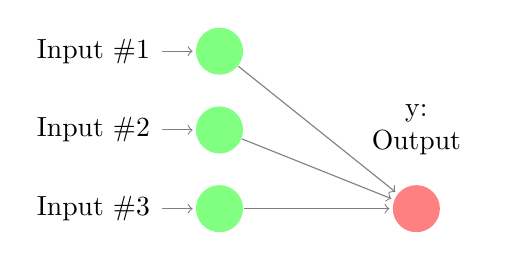
\begin{tikzpicture}[shorten >=1pt,->,draw=black!50, node distance=\layersep]
    \tikzstyle{every pin edge}=[<-,shorten <=1pt]
    \tikzstyle{neuron}=[circle,fill=black!25,minimum size=17pt,inner sep=0pt]
    \tikzstyle{input neuron}=[neuron, fill=green!50];
    \tikzstyle{output neuron}=[neuron, fill=red!50];
    \tikzstyle{annot} = [text width=4em, text centered]

    % Draw the input layer nodes
    \foreach \name / \y in {1,...,3}
    % This is the same as writing \foreach \name / \y in {1/1,2/2,3/3,4/4}
        \node[input neuron, pin=left:Input \#\y] (I-\name) at (0,-\y) {};


    % Draw the output layer node
    %\node[output neuron,pin={[pin edge={->}]right:Output}, right of=H-3] (O) {};
    \node[output neuron, right of=I-3] (O) {};

    % Connect every node in the input layer with every node in the
    % hidden layer.
    \foreach \source in {1,...,3}
            \path (I-\source) edge (O);



    % Annotate the layers
    \node[annot,above of=O, node distance=1cm] (ol) {y: Output};

\end{tikzpicture}

  \caption{Ein 1-schichtiges Perceptron, dargestellt als graphisches Modell.}
\end{figure}

Wie wir später sehen werden, kann das Perceptron auch als eine einfache Variante eines Feed-Forward-Neuronalen-Netzes mit nur einem Ausgangsneuronen, mit der Heaviside-Funktion
\begin{equation}
    \sigma = \begin{cases}
               1               & n \geq 0\\
               0               & n \leq 0
           \end{cases}
\end{equation}

als Aktivierungsfunktion interpretiert werden.

Als graphisches Modell sieht es dann aus wie Abbildung \ref{fig:SLP}. Alle Inputs gehen in den gleichen Knoten, der dann die Ausgabe mit der Formel \ref{eq:perceptron} bestimmt. 

Auf den benutzen Trainingsalgorithmus werden wir nicht eingehen, da der später betrachtete Backpropagation-Algorithmus für allgemeine ANNs auf Perceptrons übertragbar ist.

\subsection{Das XOR-Problem: nicht linear separierbare Probleme}
Es gibt viele Probleme, die von einem Perceptron nicht gelöst werden können. Es können nur linear seperierbare Funktionen von linearen Modellen approximiert werden. Da das Perceptron als Verknüfung von linearen Funktionen auch linear ist, kann auch es diese Klasse von Funktionen nicht lösen

\subsection{Die Lösung: Neuronale Netze}
Neuronale Netze sind eine Weiterentwicklung von Perceptrons. Sie besitzen noch eine(oder mehrere) weitere Schicht(en) Neuronen, die jedoch nicht nur lineare Transformationen durchführen, sondern zusätzlich noch eine nicht lineare.

Diese Nicht-linearität ermöglicht es, auch nicht linear seperierbare Probleme zu lösen - in \cite{cybenko1989approximation} wurde sogar bewiesen, dass mit ausreichend großen Netzwerken alle Funktionen approximiert werden können!

Durch die Nicht-linearität und durch die komplexere Verknüpfung resultiert ein nicht lineares Optimierungsproblem, das nicht mehr analytisch zu lösen ist. Deswegen werden numerische Verfahren benutzt.


